\section{Representation of Particles by Discrete Surfaces}\label{sec:particle-representation}

\begin{figure}[b]
    \centering
    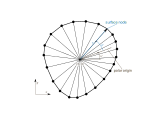
\includegraphics{img/model_development/particle_coordinates}
    \caption{Position of a Particle and Its Local Coordinate System}
    \label{fig:model_development/particle_coordinates}
\end{figure}
\begin{figure}
    \centering
    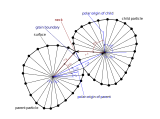
\includegraphics{img/model_development/two_particle_contact}
    \caption{Contact of Two Particles with Respective Properties}
    \label{fig:model_development/two_particle_contact}
\end{figure}

Continuous description of the particle surface geometry is only possible for nearly ideal geometries.
For complicated geometries a discretized approach is feasible.
For the current work, the concept of a node shall be introduced.
A node is here considered as a discrete point of the particle surface connected with its neighbors by straight lines.
The spline of those lines is defining the surface of the particle.

The location of each node in space is defined by a tuple of polar coordinates $(\Angle, \Radius)$, where $\Angle$ is the angle coordinate and $\Radius$ the radius resp.~distance from origin.
The origin of the polar coordinates is distinct for each particle and is considered as the center of the particle, although it is generally not identical with the barycenter of the particle.
The center of the particle is used as an anchor for defining a particle's postion in space.
With this concept the particle can be moved in space without translating the surface node coordinates and the description of node evolution is simplified, since only the local geometry must be regarded.
Particle movement occurs due to diffusional fluxes in the grain boundaries, which is macroscopically observed as shrinkage.
The location of a particle is defined by the cartesian coordinates of its center $\X$ and $\Y$, as well as a rotation angle $\RotationAngle$ with the center as pole.
The rotation angle always counts from the $\X$-axis on in mathematical direction.
The rotation angle also defines the origin axis of the particles local coordinate system.
See \autoref{fig:model_development/particle_coordinates} for illustration on this.

In regard of sintering processes, the contact properties of multiple particles are investigated.
The common interface of two particles in contact is commonly called a sinter neck.
It consists of a grain boundary bounded by the triple points between the grain boundary and the two adjacent free surfaces.
\autoref{fig:model_development/two_particle_contact} shows such a contact of two particles.
Until here, three types of nodes can be identified:
\begin{description}
    \item[Surface Nodes] forming the free surface of a particle in contact to atmosphere or vacuum (black).
    \item[Grain Boundary Nodes] forming the grain boundary in a particle contact (dark blue).
    \item[Neck Nodes] representing the triple point between grain boundary and two surfaces (dark red).
\end{description}
Details on the conditions at those nodes are given in the following sections.
Since every particle has its own polar coordinate system, the node coordinates involved can be regarded in either the one's or the other's coordinate system.
The coordinate system used shall be denoted hereinafter by $\ldots^{|\ldots}$ superscripts where necessary as done in \autoref{fig:model_development/two_particle_contact}.
As example, the coordinates of one neck node are shown in the figure as $(\Angle^{\Regarding 1}, \Radius^{\Regarding 1})$ and $(\Angle^{\Regarding 2}, \Radius^{\Regarding 2})$.
Note, that both tuples represent the same point in global space.
